%========================================
% LESSON CONTENT: Sistema de Coordenadas
%========================================

\lesson{Sistema de Coordenadas Rectangulares}

%========================================
% SECTION 10.1: Sistema de Coordenadas Rectangulares
%========================================
\subsectiontitle{Introducción al Sistema de Coordenadas}

\begin{definition}
\textbf{Sistema de Coordenadas Rectangulares (o Cartesiano):}

El sistema de coordenadas rectangulares está formado por dos rectas numéricas perpendiculares:

\begin{itemize}[leftmargin=*]
    \item \textbf{Eje $x$ (eje horizontal):} Representa la recta horizontal
    \item \textbf{Eje $y$ (eje vertical):} Representa la recta vertical
    \item \textbf{Origen:} El punto de intersección de los ejes, denotado por $O = (0, 0)$
    \item \textbf{Cuadrantes:} Los ejes dividen el plano en cuatro regiones, numeradas en sentido antihorario como I, II, III y IV
\end{itemize}
\end{definition}

% Visual representation of the Cartesian Plane with all four quadrants
\begin{center}
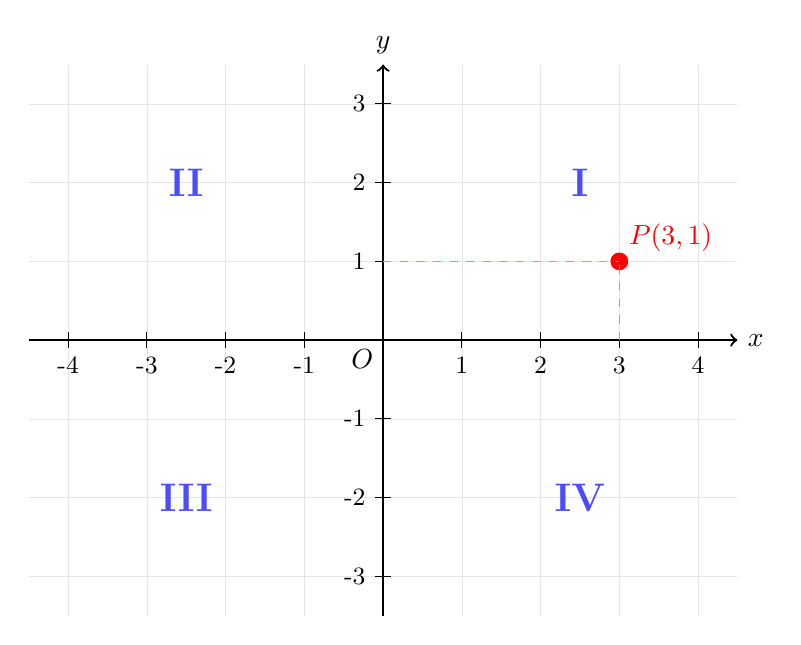
\begin{tikzpicture}[scale=1.0]
    % Grid (optional, light gray)
    \draw[gray!20, very thin] (-4.5,-3.5) grid (4.5,3.5);

    % Axes
    \draw[->, thick] (-4.5,0) -- (4.5,0) node[right] {$x$};
    \draw[->, thick] (0,-3.5) -- (0,3.5) node[above] {$y$};

    % Origin label
    \node[below left] at (0,0) {$O$};

    % Axis labels
    \foreach \x in {-4,-3,-2,-1,1,2,3,4}
        \draw (\x,0.1) -- (\x,-0.1) node[below, font=\small] {\x};
    \foreach \y in {-3,-2,-1,1,2,3}
        \draw (0.1,\y) -- (-0.1,\y) node[left, font=\small] {\y};

    % Quadrant labels
    \node[blue!70, font=\Large\bfseries] at (2.5,2) {I};
    \node[blue!70, font=\Large\bfseries] at (-2.5,2) {II};
    \node[blue!70, font=\Large\bfseries] at (-2.5,-2) {III};
    \node[blue!70, font=\Large\bfseries] at (2.5,-2) {IV};

    % Example point
    \filldraw[red] (3,1) circle (3pt);
    \node[red, above right] at (3,1) {$P(3,1)$};

    % Dashed lines to show coordinates
    \draw[dashed, red!50] (3,0) -- (3,1);
    \draw[dashed, red!50] (0,1) -- (3,1);
\end{tikzpicture}
\end{center}

\begin{definition}
\textbf{Par Ordenado:}

Un par ordenado $(a, b)$ representa un punto sobre el sistema de coordenadas y está formado por dos números denominados componentes:

\begin{itemize}
    \item \textbf{Primera componente ($a$):} Representa el desplazamiento horizontal sobre el eje $x$ (abscisa)
    \item \textbf{Segunda componente ($b$):} Representa el desplazamiento vertical sobre el eje $y$ (ordenada)
\end{itemize}

\textbf{Nota importante:} El orden de las componentes es crucial. $(a, b) \neq (b, a)$ a menos que $a = b$.
\end{definition}

% Visual guide for signs in each quadrant
\begin{center}
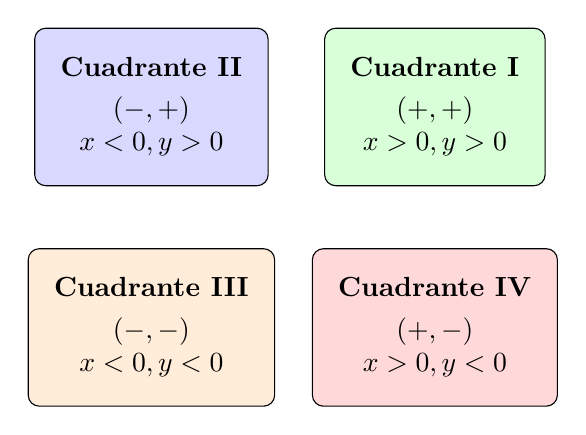
\begin{tikzpicture}[scale=0.8]
    % Quadrant I (upper right)
    \node[draw, fill=green!15, minimum width=2.5cm, minimum height=2cm, rounded corners] at (4.5,0) {
        \begin{tabular}{c}
            \textbf{Cuadrante I} \\[0.1cm]
            $(+, +)$ \\
            $x > 0, y > 0$
        \end{tabular}
    };

    % Quadrant II (upper left)
    \node[draw, fill=blue!15, minimum width=2.5cm, minimum height=2cm, rounded corners] at (0,0) {
        \begin{tabular}{c}
            \textbf{Cuadrante II} \\[0.1cm]
            $(-, +)$ \\
            $x < 0, y > 0$
        \end{tabular}
    };

    % Quadrant III (lower left)
    \node[draw, fill=orange!15, minimum width=2.5cm, minimum height=2cm, rounded corners] at (0,-3.5) {
        \begin{tabular}{c}
            \textbf{Cuadrante III} \\[0.1cm]
            $(-, -)$ \\
            $x < 0, y < 0$
        \end{tabular}
    };

    % Quadrant IV (lower right)
    \node[draw, fill=red!15, minimum width=2.5cm, minimum height=2cm, rounded corners] at (4.5,-3.5) {
        \begin{tabular}{c}
            \textbf{Cuadrante IV} \\[0.1cm]
            $(+, -)$ \\
            $x > 0, y < 0$
        \end{tabular}
    };
\end{tikzpicture}
\end{center}

\begin{example}
\textbf{Localización de Puntos:}

Para localizar el punto correspondiente al par ordenado $(3, 1)$:
\begin{enumerate}
    \item Desplácese 3 unidades a la \textbf{derecha} a partir del origen, a lo largo del eje $x$
    \item Luego desplácese 1 unidad hacia \textbf{arriba}, en forma paralela al eje $y$
\end{enumerate}

El punto $(3, 1)$ se encuentra en el \textbf{Cuadrante I}.
\end{example}

\newpage

\begin{example}
\textbf{Ubicación de Varios Puntos:}

Grafique los siguientes puntos en el plano cartesiano: $A(2, 3)$, $B(-4, 2)$, $C(-3, -2)$, $D(4, -1)$, $E(0, 3)$, $F(-2, 0)$

\begin{center}
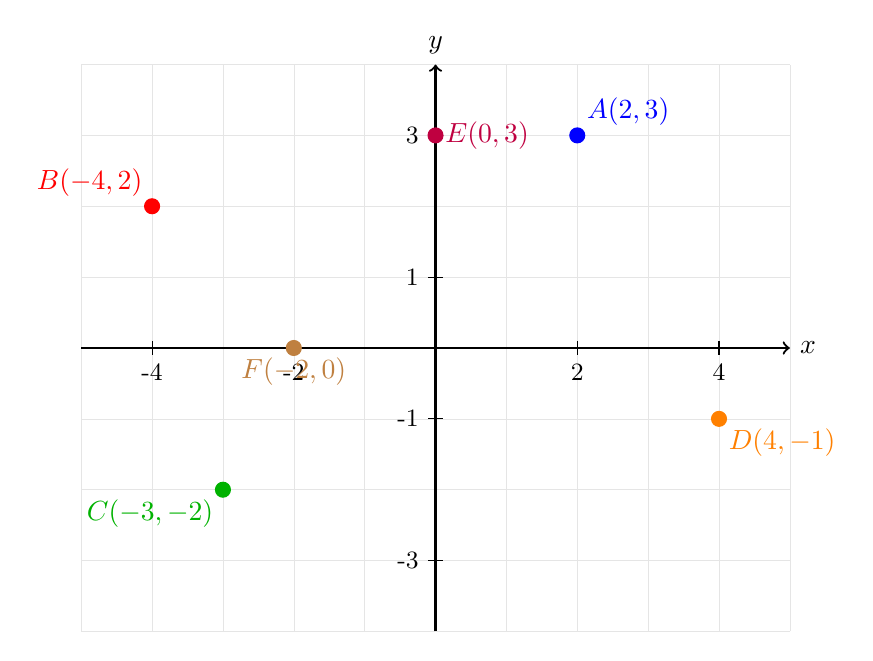
\begin{tikzpicture}[scale=0.9]
    % Grid
    \draw[gray!20, very thin] (-5,-4) grid (5,4);

    % Axes
    \draw[->, thick] (-5,0) -- (5,0) node[right] {$x$};
    \draw[->, thick] (0,-4) -- (0,4) node[above] {$y$};

    % Axis labels
    \foreach \x in {-4,-2,2,4}
        \draw (\x,0.1) -- (\x,-0.1) node[below, font=\small] {\x};
    \foreach \y in {-3,-1,1,3}
        \draw (0.1,\y) -- (-0.1,\y) node[left, font=\small] {\y};

    % Points
    \filldraw[blue] (2,3) circle (3pt);
    \node[blue, above right] at (2,3) {$A(2,3)$};

    \filldraw[red] (-4,2) circle (3pt);
    \node[red, above left] at (-4,2) {$B(-4,2)$};

    \filldraw[green!70!black] (-3,-2) circle (3pt);
    \node[green!70!black, below left] at (-3,-2) {$C(-3,-2)$};

    \filldraw[orange] (4,-1) circle (3pt);
    \node[orange, below right] at (4,-1) {$D(4,-1)$};

    \filldraw[purple] (0,3) circle (3pt);
    \node[purple, right] at (0,3) {$E(0,3)$};

    \filldraw[brown] (-2,0) circle (3pt);
    \node[brown, below] at (-2,0) {$F(-2,0)$};
\end{tikzpicture}
\end{center}

\textbf{Observaciones:}
\begin{itemize}
    \item Punto $A(2, 3)$ está en el Cuadrante I
    \item Punto $B(-4, 2)$ está en el Cuadrante II
    \item Punto $C(-3, -2)$ está en el Cuadrante III
    \item Punto $D(4, -1)$ está en el Cuadrante IV
    \item Punto $E(0, 3)$ está sobre el eje $y$ (no pertenece a ningún cuadrante)
    \item Punto $F(-2, 0)$ está sobre el eje $x$ (no pertenece a ningún cuadrante)
\end{itemize}
\end{example}

%========================================
% SECTION 10.2: Fórmula de Distancia
%========================================
\subsectiontitle{Fórmula de Distancia}

La distancia entre dos puntos en el plano cartesiano puede calcularse usando el teorema de Pitágoras.

\begin{definition}
\textbf{Fórmula de Distancia:}

La distancia $d$ entre los puntos $(x_1, y_1)$ y $(x_2, y_2)$ está dada por:

$$\boxed{d = \sqrt{(x_2 - x_1)^2 + (y_2 - y_1)^2}}$$

Esta fórmula se deriva del teorema de Pitágoras aplicado al triángulo rectángulo formado por los dos puntos.
\end{definition}

% Visual proof using right triangle
\begin{center}
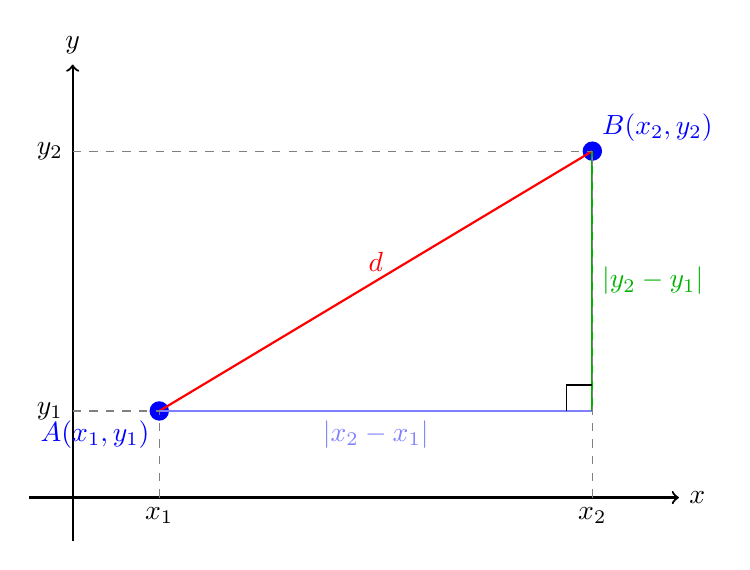
\begin{tikzpicture}[scale=1.1]
    % Axes
    \draw[->, thick] (-0.5,0) -- (7,0) node[right] {$x$};
    \draw[->, thick] (0,-0.5) -- (0,5) node[above] {$y$};

    % Points
    \def\xa{1}
    \def\ya{1}
    \def\xb{6}
    \def\yb{4}

    \filldraw[blue] (\xa,\ya) circle (3pt);
    \node[blue, below left] at (\xa,\ya) {$A(x_1, y_1)$};

    \filldraw[blue] (\xb,\yb) circle (3pt);
    \node[blue, above right] at (\xb,\yb) {$B(x_2, y_2)$};

    % Right triangle
    \draw[thick, red] (\xa,\ya) -- (\xb,\yb);
    \node[red, above, sloped] at ({(\xa+\xb)/2},{(\ya+\yb)/2}) {$d$};

    \draw[thick, blue!50] (\xa,\ya) -- (\xb,\ya);
    \node[blue!50, below] at ({(\xa+\xb)/2},\ya) {$|x_2 - x_1|$};

    \draw[thick, green!70!black] (\xb,\ya) -- (\xb,\yb);
    \node[green!70!black, right] at (\xb,{(\ya+\yb)/2}) {$|y_2 - y_1|$};

    % Right angle mark
    \draw (\xb-0.3,\ya) -- (\xb-0.3,\ya+0.3) -- (\xb,\ya+0.3);

    % Dashed lines to axes
    \draw[dashed, gray] (\xa,0) -- (\xa,\ya);
    \draw[dashed, gray] (\xb,0) -- (\xb,\yb);
    \draw[dashed, gray] (0,\ya) -- (\xa,\ya);
    \draw[dashed, gray] (0,\yb) -- (\xb,\yb);

    % Axis labels
    \node[below] at (\xa,0) {$x_1$};
    \node[below] at (\xb,0) {$x_2$};
    \node[left] at (0,\ya) {$y_1$};
    \node[left] at (0,\yb) {$y_2$};
\end{tikzpicture}
\end{center}

\textbf{Por el Teorema de Pitágoras:}
$$d^2 = (x_2 - x_1)^2 + (y_2 - y_1)^2$$

Tomando la raíz cuadrada de ambos lados:
$$d = \sqrt{(x_2 - x_1)^2 + (y_2 - y_1)^2}$$

\begin{example}
\textbf{Ejemplo 1: Calcular la distancia entre dos puntos}

Calcule la distancia entre los puntos $(-3, 5)$ y $(6, 4)$.

\textbf{Solución:}

Tomamos $(x_1, y_1) = (-3, 5)$ y $(x_2, y_2) = (6, 4)$.

\textbf{Nota:} El orden en que se consideren los puntos no altera el resultado final.

Identificamos las componentes:
\begin{itemize}
    \item $x_1 = -3$
    \item $y_1 = 5$
    \item $x_2 = 6$
    \item $y_2 = 4$
\end{itemize}

Reemplazando valores en la fórmula de distancia:
\begin{align*}
d &= \sqrt{(x_2 - x_1)^2 + (y_2 - y_1)^2} \\
  &= \sqrt{(6 - (-3))^2 + (4 - 5)^2} \\
  &= \sqrt{(6 + 3)^2 + (-1)^2} \\
  &= \sqrt{9^2 + (-1)^2} \\
  &= \sqrt{81 + 1} \\
  &= \sqrt{82}
\end{align*}

\textbf{Respuesta:} La distancia entre los puntos es $\sqrt{82} \approx 9.06$ unidades.
\end{example}

\begin{center}
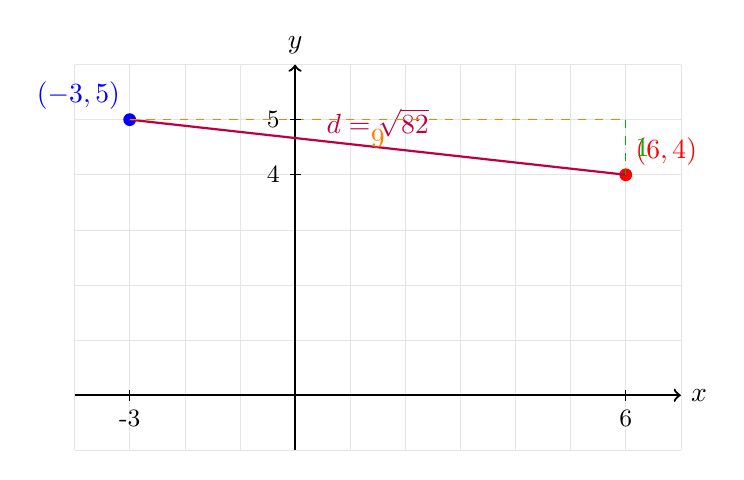
\begin{tikzpicture}[scale=0.7]
    % Grid
    \draw[gray!20, very thin] (-4,-1) grid (7,6);

    % Axes
    \draw[->, thick] (-4,0) -- (7,0) node[right] {$x$};
    \draw[->, thick] (0,-1) -- (0,6) node[above] {$y$};

    % Points
    \filldraw[blue] (-3,5) circle (3pt);
    \node[blue, above left] at (-3,5) {$(-3,5)$};

    \filldraw[red] (6,4) circle (3pt);
    \node[red, above right] at (6,4) {$(6,4)$};

    % Distance line
    \draw[thick, purple] (-3,5) -- (6,4);
    \node[purple, above, sloped] at (1.5,4.5) {$d = \sqrt{82}$};

    % Right triangle
    \draw[dashed, orange] (-3,5) -- (6,5);
    \draw[dashed, green!70!black] (6,5) -- (6,4);

    \node[orange, below] at (1.5,5) {$9$};
    \node[green!70!black, right] at (6,4.5) {$1$};

    % Axis labels
    \foreach \x in {-3,6}
        \draw (\x,0.1) -- (\x,-0.1) node[below, font=\small] {\x};
    \foreach \y in {4,5}
        \draw (0.1,\y) -- (-0.1,\y) node[left, font=\small] {\y};
\end{tikzpicture}
\end{center}

\newpage

\begin{example}
\textbf{Ejemplo 2: Verificar si un triángulo es rectángulo}

Determine si el triángulo con vértices $A(1, 1)$, $B(4, 5)$, y $C(6, 2)$ es un triángulo rectángulo.

\textbf{Solución:}

Usamos el teorema de Pitágoras: Si $a^2 + b^2 = c^2$, el triángulo es rectángulo.

Primero calculamos las longitudes de los tres lados:

\textbf{Lado AB:}
\begin{align*}
d_{AB} &= \sqrt{(4-1)^2 + (5-1)^2} \\
       &= \sqrt{3^2 + 4^2} \\
       &= \sqrt{9 + 16} \\
       &= \sqrt{25} = 5
\end{align*}

\textbf{Lado BC:}
\begin{align*}
d_{BC} &= \sqrt{(6-4)^2 + (2-5)^2} \\
       &= \sqrt{2^2 + (-3)^2} \\
       &= \sqrt{4 + 9} \\
       &= \sqrt{13}
\end{align*}

\textbf{Lado AC:}
\begin{align*}
d_{AC} &= \sqrt{(6-1)^2 + (2-1)^2} \\
       &= \sqrt{5^2 + 1^2} \\
       &= \sqrt{25 + 1} \\
       &= \sqrt{26}
\end{align*}

\textbf{Verificación:}

Comprobamos si $(d_{AB})^2 + (d_{BC})^2 = (d_{AC})^2$:
$$5^2 + (\sqrt{13})^2 = 25 + 13 = 38$$
$$(\sqrt{26})^2 = 26$$

Como $38 \neq 26$, probamos otra combinación:
$$(\sqrt{13})^2 + (\sqrt{26})^2 = 13 + 26 = 39$$
$$5^2 = 25$$

Como $39 \neq 25$, el triángulo \textbf{NO es rectángulo}.
\end{example}

%========================================
% SECTION 10.3: Fórmula del Punto Medio
%========================================
\subsectiontitle{Fórmula del Punto Medio}

El punto medio de un segmento de recta es el punto que se encuentra exactamente a la mitad del camino entre los dos extremos.

\begin{definition}
\textbf{Fórmula del Punto Medio:}

Las coordenadas del punto medio $M$ del segmento con extremos $(x_1, y_1)$ y $(x_2, y_2)$ se determinan mediante:

$$\boxed{M = \left(\frac{x_1 + x_2}{2}, \frac{y_1 + y_2}{2}\right)}$$

Es decir:
\begin{itemize}
    \item La coordenada $x$ del punto medio es el \textbf{promedio} de las coordenadas $x$ de los extremos
    \item La coordenada $y$ del punto medio es el \textbf{promedio} de las coordenadas $y$ de los extremos
\end{itemize}
\end{definition}

% Visual representation of midpoint
\begin{center}
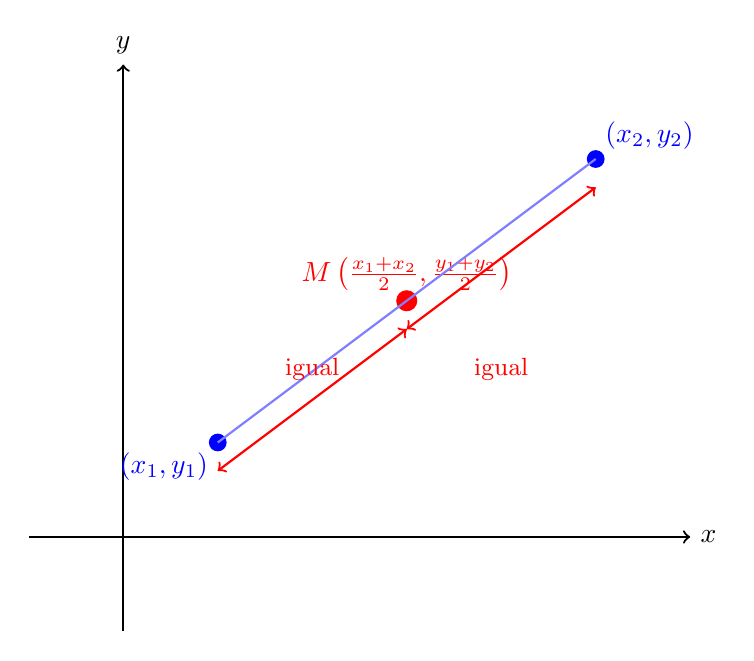
\begin{tikzpicture}[scale=1.2]
    % Axes
    \draw[->, thick] (-1,0) -- (6,0) node[right] {$x$};
    \draw[->, thick] (0,-1) -- (0,5) node[above] {$y$};

    % Points
    \pgfmathsetmacro{\xa}{1}
    \pgfmathsetmacro{\ya}{1}
    \pgfmathsetmacro{\xb}{5}
    \pgfmathsetmacro{\yb}{4}
    \pgfmathsetmacro{\xm}{(\xa+\xb)/2}
    \pgfmathsetmacro{\ym}{(\ya+\yb)/2}

    \filldraw[blue] (\xa,\ya) circle (2.5pt);
    \node[blue, below left] at (\xa,\ya) {$(x_1, y_1)$};

    \filldraw[blue] (\xb,\yb) circle (2.5pt);
    \node[blue, above right] at (\xb,\yb) {$(x_2, y_2)$};

    \filldraw[red] (\xm,\ym) circle (3pt);
    \node[red, above] at (\xm,\ym) {$M\left(\frac{x_1+x_2}{2}, \frac{y_1+y_2}{2}\right)$};

    % Line segment
    \draw[thick, blue!50] (\xa,\ya) -- (\xb,\yb);

    % Equal distance marks
    \draw[<->, red, thick] (\xa,\ya-0.3) -- (\xm,\ym-0.3);
    \draw[<->, red, thick] (\xm,\ym-0.3) -- (\xb,\yb-0.3);
    \node[red, below] at ({(\xa+\xm)/2},\ym-0.5) {\small igual};
    \node[red, below] at ({(\xm+\xb)/2},\ym-0.5) {\small igual};
\end{tikzpicture}
\end{center}

\begin{example}
\textbf{Ejemplo 1: Encontrar el punto medio}

Encuentre las coordenadas del punto medio del segmento con extremos $(8, -4)$ y $(-9, 6)$.

\textbf{Solución:}

Tomamos $(x_1, y_1) = (8, -4)$ y $(x_2, y_2) = (-9, 6)$.

\textbf{Nota:} El orden en que se consideren los puntos no altera el resultado final.

Identificamos las componentes:
\begin{itemize}
    \item $x_1 = 8$
    \item $y_1 = -4$
    \item $x_2 = -9$
    \item $y_2 = 6$
\end{itemize}

Aplicando la fórmula del punto medio:
\begin{align*}
M &= \left(\frac{x_1 + x_2}{2}, \frac{y_1 + y_2}{2}\right) \\
  &= \left(\frac{8 + (-9)}{2}, \frac{-4 + 6}{2}\right) \\
  &= \left(\frac{-1}{2}, \frac{2}{2}\right) \\
  &= \left(-\frac{1}{2}, 1\right)
\end{align*}

\textbf{Respuesta:} El punto medio es $M\left(-\frac{1}{2}, 1\right)$ o $M(-0.5, 1)$.
\end{example}

\begin{center}
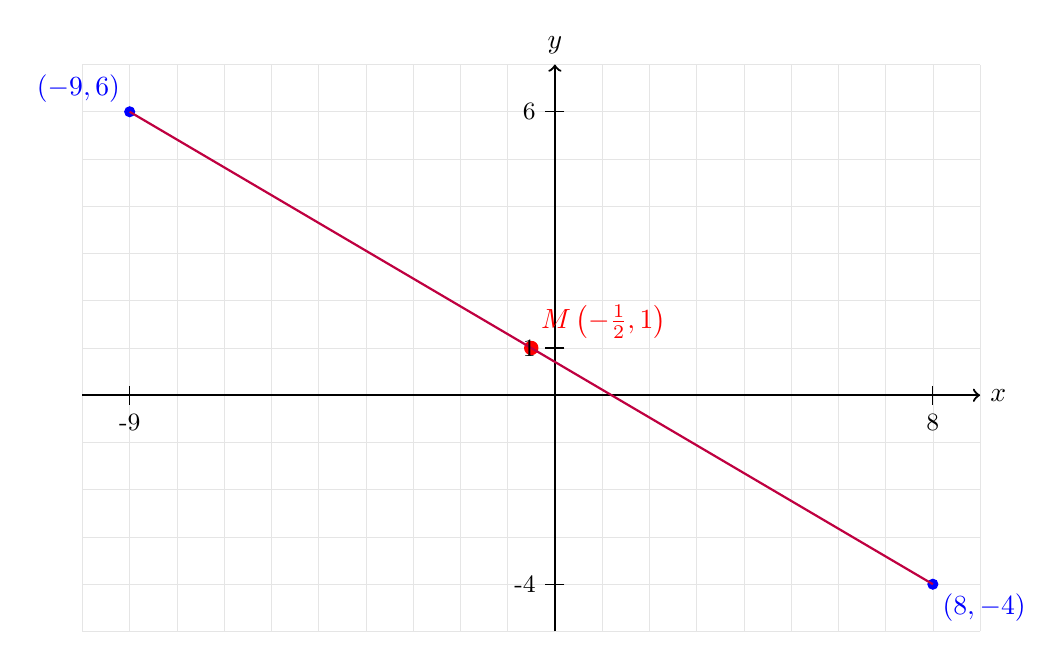
\begin{tikzpicture}[scale=0.6]
    % Grid
    \draw[gray!20, very thin] (-10,-5) grid (9,7);

    % Axes
    \draw[->, thick] (-10,0) -- (9,0) node[right] {$x$};
    \draw[->, thick] (0,-5) -- (0,7) node[above] {$y$};

    % Points
    \filldraw[blue] (8,-4) circle (3pt);
    \node[blue, below right] at (8,-4) {$(8,-4)$};

    \filldraw[blue] (-9,6) circle (3pt);
    \node[blue, above left] at (-9,6) {$(-9,6)$};

    \filldraw[red] (-0.5,1) circle (4pt);
    \node[red, above right] at (-0.5,1) {$M\left(-\frac{1}{2},1\right)$};

    % Line segment
    \draw[thick, purple] (8,-4) -- (-9,6);

    % Axis labels
    \foreach \x in {-9,8}
        \draw (\x,0.2) -- (\x,-0.2) node[below, font=\small] {\x};
    \foreach \y in {-4,1,6}
        \draw (0.2,\y) -- (-0.2,\y) node[left, font=\small] {\y};
\end{tikzpicture}
\end{center}

\newpage

\begin{example}
\textbf{Ejemplo 2: Encontrar un extremo dado el punto medio}

El punto medio de un segmento es $M(3, 5)$ y uno de sus extremos es $A(1, 2)$. Encuentre las coordenadas del otro extremo $B$.

\textbf{Solución:}

Sea $B(x, y)$ el extremo desconocido. Sabemos que:
$$M = \left(\frac{x_1 + x}{2}, \frac{y_1 + y}{2}\right) = (3, 5)$$

donde $(x_1, y_1) = (1, 2)$.

Para la coordenada $x$:
\begin{align*}
\frac{1 + x}{2} &= 3 \\
1 + x &= 6 \\
x &= 5
\end{align*}

Para la coordenada $y$:
\begin{align*}
\frac{2 + y}{2} &= 5 \\
2 + y &= 10 \\
y &= 8
\end{align*}

\textbf{Respuesta:} El otro extremo es $B(5, 8)$.

\textbf{Verificación:}
$$M = \left(\frac{1 + 5}{2}, \frac{2 + 8}{2}\right) = \left(\frac{6}{2}, \frac{10}{2}\right) = (3, 5)$$ \checkmark
\end{example}

\begin{theorem}
\textbf{Propiedades Importantes:}

\begin{enumerate}
    \item La distancia siempre es un valor \textbf{positivo} o cero: $d \geq 0$
    \item La distancia de un punto a sí mismo es cero: $d(P, P) = 0$
    \item La distancia es \textbf{simétrica}: $d(A, B) = d(B, A)$
    \item El punto medio siempre está entre los dos extremos
    \item El punto medio divide al segmento en dos partes de igual longitud
\end{enumerate}
\end{theorem}

\textbf{Resumen de Fórmulas:}

\begin{center}
\begin{tikzpicture}
    % Distance formula box
    \node[draw, fill=blue!10, text width=6.5cm, minimum height=2.2cm, rounded corners] at (0,0) {
        \textbf{Fórmula de Distancia} \\[0.3cm]
        $d = \sqrt{(x_2 - x_1)^2 + (y_2 - y_1)^2}$ \\[0.2cm]
        \small Calcula la distancia entre dos puntos
    };

    % Midpoint formula box
    \node[draw, fill=green!10, text width=6.5cm, minimum height=2.2cm, rounded corners] at (0,-3) {
        \textbf{Fórmula del Punto Medio} \\[0.3cm]
        $M = \left(\dfrac{x_1 + x_2}{2}, \dfrac{y_1 + y_2}{2}\right)$ \\[0.2cm]
        \small Encuentra el punto medio de un segmento
    };
\end{tikzpicture}
\end{center}
